\documentclass[11pt]{article}
\pdfminorversion=7
\usepackage[T1]{fontenc}
\usepackage{lmodern}
\usepackage{amsmath,amssymb,booktabs,graphicx,geometry,hyperref,xcolor,array,enumitem,listings}
\usepackage[most]{tcolorbox}
\geometry{margin=25mm}
\hypersetup{colorlinks=true,linkcolor=blue!55!black,urlcolor=blue!55!black,citecolor=blue!55!black}
\newcommand{\src}[1]{\texttt{#1}}
\newcommand{\ma}[1]{\mathbf{#1}}
\newcommand{\ve}[1]{\boldsymbol{#1}}
\newcommand{\E}{\operatorname{E}}
\newcommand{\Cov}{\operatorname{Cov}}
\newcommand{\Var}{\operatorname{Var}}
\setlist{itemsep=2pt,topsep=4pt}
\lstset{language=Fortran,basicstyle=\ttfamily\small,columns=fullflexible,keepspaces=true,
  frame=single,rulecolor=\color{black!25},backgroundcolor=\color{black!3},xleftmargin=4pt,xrightmargin=4pt,
  commentstyle=\color{black!55},keywordstyle=\color{blue!45!black},breaklines=true,showstringspaces=false}
\newtcolorbox{question}[1]{colback=blue!3!white,colframe=blue!35!black,boxrule=0.5pt,arc=2pt,
  left=6pt,right=6pt,top=4pt,bottom=4pt,fonttitle=\bfseries,title=#1}
\newtcolorbox{recommend}{colback=green!4!white,colframe=green!35!black,boxrule=0.5pt,arc=2pt,
  left=6pt,right=6pt,top=4pt,bottom=4pt,fonttitle=\bfseries,title=Our recommendation}

\title{SelAction: open questions on the model\\[4pt]
\large Background, equations, numerical evidence and recommendations\\
for Piter Bijma and Jack Dekkers}
\author{Austin Putz}
\date{2 October 2026}

\begin{document}
\maketitle

\begin{abstract}
We have been bringing the SelAction Fortran code (Rutten and Bijma) up to date, writing a regression test suite for it, and writing a technical report that ties every equation to the routine that computes it. That work turned up places where we cannot tell from the code alone what the intended model is. For each question, we describe the relevant code, the alternative we considered, any measured effect, and our recommendation. Model changes raised as questions have not been made. Numerical safeguards that prevented valid selection have already been removed; other programming corrections are listed briefly in Appendix~\ref{app:fixed}.
\end{abstract}

\tableofcontents

%======================================================================
\section{Purpose and how to read this}

We have made each section self-contained so that you can review the questions without reopening the source. The questions concern selection-index and inbreeding theory as well as implementation choices; we would value both of your views.

Table~\ref{tab:summary} lists the questions. Where an effect is quantified, it is the largest change in the examples we ran, not a general bound.

\begin{table}[ht]
\centering\small
\caption{Summary of the open questions.}\label{tab:summary}
\begin{tabular}{>{\raggedright}p{.03\linewidth}>{\raggedright}p{.30\linewidth}>{\raggedright}p{.30\linewidth}>{\raggedright\arraybackslash}p{.27\linewidth}}
\toprule
& Question & Evidence or effect in examples & Recommendation\\\midrule
\multicolumn{4}{l}{\emph{Overlapping generations}}\\
1 & Definition of the generation interval & Original source uses the stated definition; no alternative model tested & Confirm age-class interpretation\\
2 & Genetic lag between age classes: per-sex path response or population trend? & $<1$\% of response in our examples; grows with more age classes & Use the population trend; please confirm\\
3 & Former $\pm1.5$\,SD search range and $\pm3$\,SD clamp (already removed) & Could select 67.5 sires when 10 were requested & Confirm removal\\
4 & No family-structure correction of intensity despite the program description & not measured & How should it be applied?\\
\multicolumn{4}{l}{\emph{Multistage selection}}\\
5 & $r_{13\mid2}=0$ and the 0.93 cap on stage correlations & up to 5.3\% of stage-3 response & Compute $r_{13\mid2}$; keep the cap for now\\
6 & Half-sib information in earlier stages when each sire has one dam; size of half-sib groups & 5.6\% of stage-1 response & Apply the same rule at all stages; clarify group sizes\\
\multicolumn{4}{l}{\emph{Rate of inbreeding}}\\
7 & Hard switch in the inbreeding correction at 20 sires & 4.590\% to 4.682\% $\Delta F$ from 19 to 20 sires in one example & Retain published $1/M_s$; examine switch\\
\bottomrule
\end{tabular}
\end{table}

Section~\ref{sec:background} summarises the state of the code and what has been changed so far. Sections~\ref{sec:ovlp}--\ref{sec:inbreeding} contain the questions. Section~\ref{sec:numerics} lists numerical points that need no decision but that you may want to know about. The source of record is \src{fortran\_mac/} at commit \src{dbdd69f} of the repository; the full mathematical description is in \src{docs/SelAction\_Technical\_Report.pdf}, which uses the same notation.

%======================================================================
\section{Background}\label{sec:background}

\subsection{The code and how it has been checked}
The working copy is \src{fortran\_mac/}. It started as a copy of \src{fortran\_linux/}, an earlier fork of the original code (\src{fortran\_orig/}, kept unchanged for reference) with the changes needed to compile with a current gfortran and some crash fixes. All changes are recorded in \src{NEWS.md}. A set of seven regression inputs with stored outputs covers one-, two- and three-stage selection, BLUP, the group information sources, and overlapping generations with and without groups. Changes are checked against these fixtures and under a debug build with floating-point traps, bounds checks, and initialization sentinels.

\subsection{Notation}
We follow the technical report. For sex $g\in\{s,d\}$: $M_s,M_d$ selected sires and dams; $d=M_d/M_s$; $p_g$ selected fraction; $t$ the truncation point, $i=\phi(t)/p$ the intensity and $k=i(i-t)$ the variance reduction; $V_I$, $r_{IH}$ index variance and accuracy; $H=\ve v^{\mathsf T}\ve A$ the breeding goal. Under overlapping generations, $K$ age classes per sex, $N_{g,c}$ candidates and $n_{g,c}$ selected in class $c$, and $w_{g,c}=n_{g,c}/\sum_c n_{g,c}$.

\subsection{Changes to results so far}
The following corrections change the program's predictions. Items 1, 2 and 4 correct defects of the original code. Item 3 corrects an error introduced in the modernized fork; the original source computes the interval correctly.
\begin{enumerate}
\item \textbf{Overlapping generations: truncation-point search.} The Ridders search for the common truncation point covered only $\pm1.5$ index standard deviations, so at least 6.7\% of the youngest class was always selected; with 10 sires from 1500 candidates the program selected 67.5. Now $\pm8$ standard deviations (Question~3).
\item \textbf{Overlapping generations: normal tail and clamp.} The univariate normal tail used Gauss--Hermite quadrature, which is inaccurate beyond about 4 standard deviations, and the standardised truncation point was clamped to $\pm3$, which forced at least 0.135\% of every age class to be selected. The tail now uses \src{erfc} and the clamp is gone (Question~3).
\item \textbf{Overlapping generations: generation interval.} A variable-renaming error in the modernized fork changed an accumulation into an assignment. It is corrected and now matches the original source (Question~1).
\item \textbf{Multistage selection: quadrature tables.} The two- and three-dimensional normal integrals use Dutt's representation \cite{dutt1973} with Gauss--Hermite quadrature, refined adaptively from 10 to 30 points. The tables of nodes and weights stopped at 20 points, so beyond 20 the integral came out as exactly 0.25 (two dimensions) or 0.125 (three) and was accepted as converged. With small selected fractions and highly correlated stages this gave grossly wrong responses (in one two-stage example a sire response of 0.6 instead of 19.9 economic units). The tables now go to 30 points.
\end{enumerate}

%======================================================================
\section{Overlapping generations}\label{sec:ovlp}

\subsection{How the program models overlapping generations}
Each sex has $K$ age classes; class 1 are the youngest candidates, born from the current parents. Each class has its own index, built from the information available at that age, with variance $V_{I,g,c}$. In ``threshold'' mode one truncation point $x_g$ per sex is applied to all classes of that sex. Because older classes were born earlier they have a lower genetic mean, $m_{g,c}$ below the youngest, and the number selected from each class is
\begin{equation}\label{eq:agecount}
n_{g,c}=N_{g,c}\,\bar\Phi\!\left(\frac{x_g-m_{g,c}}{\sqrt{V_{I,g,c}}}\right),\qquad
\sum_c n_{g,c}=M_g .
\end{equation}
In ``specified-count'' mode the $n_{g,c}$ are inputs. The selection differential of each path is the weighted mean of the class differentials, and the annual response follows Rendel and Robertson \cite{rendel1950}:
\begin{equation}\label{eq:rr}
\Delta G^{\mathrm{year}}=\frac{S_s+S_d}{L_s+L_d},\qquad
S_g=\sum_c w_{g,c}\,i_{g,c}\sqrt{V_{I,g,c}} .
\end{equation}
The program writes this as $\tfrac12(\Delta H_s^{\mathrm{year}}+\Delta H_d^{\mathrm{year}})$ with $\Delta H_g^{\mathrm{year}}=S_g/L$ and $L=\tfrac12(L_s+L_d)$, which is the same thing. It then updates the genetic covariances of each class for the Bulmer effect and mixes the classes of each sex, adding the variance between the means of the selected animals of different classes (law of total variance). This is repeated for 25 rounds.

\subsection{Question 1: the generation interval}
The program uses the mean age-class number of selected parents as its interval,
\begin{equation}\label{eq:interval}
L_g=\sum_c c\,w_{g,c},\qquad L=\tfrac12(L_s+L_d),
\end{equation}
with the youngest class at age 1. The original \src{fortran\_orig/selovlp.f90} accumulates the contributions from all age classes correctly. (As distributed it does not compile with a current gfortran, because \src{genint} is used without being declared under \texttt{implicit none}.) When the fork introduced local variables to make it compile, one renamed variable turned the accumulation into an assignment, so only the oldest active class's term was kept (added, in threshold mode, to a stale value left by \src{trunc\_delta}). This distorted annual response and the covariance mixture. The error is fixed in \src{fortran\_mac/}; it is not a defect in the original model. In the corrected \src{ovlp2} and \src{ovlpgrp} examples, direct calculation from the printed selected counts gives $L=1.040$ and $L=1.014$, respectively, matching the code.

\begin{question}{Question 1}
Does the age-class numbering in Eq.~\eqref{eq:interval} represent actual parental ages, with the youngest class at age 1 and each subsequent class one cohort interval older? If age at first offspring differs from one cohort interval, should users account for it outside SelAction?
\end{question}
\begin{recommend}
Keep Eq.~\eqref{eq:interval} as implemented in the original source, and clarify the age units in user documentation.
\end{recommend}

\subsection{Question 2: the genetic lag between age classes}\label{sec:lag}
At equilibrium every cohort of candidates is better than the cohort born one interval earlier by the population's annual genetic gain, $\Delta G^{\mathrm{year}}$ of Eq.~\eqref{eq:rr}. Male and female candidates born in the same year descend from the same parents, so their expected means are the same, and the mean of class $c$ relative to class 1 should be $-(c-1)\Delta G^{\mathrm{year}}$ for both sexes \cite{hill1974}. The program instead uses each sex's own path response:
\begin{lstlisting}
! trunc_delta (selroutines.f90): class means for the threshold search
tmean(p)=tmean(1)-((p-1)*stotalresponse)                ! sires
tmean(p)=tmean(nclass+1)-((p-nclass-1)*dtotalresponse)  ! dams
! ovlp (selovlp.f90): breeding values of the selected, for the covariance mixture
mean(q,p)=tempresponse-(q*sresponse(p)) !let op
mean(q,p)=tempresponse-((q-nclass)*dresponse(p)) !let op
\end{lstlisting}
Here \src{stotalresponse} is $\Delta H_s^{\mathrm{year}}=S_s/L$, twice the sire path's contribution to the population gain, not a rate of change of any cohort mean. The source flags these assignments with \emph{let op} (``note'') comments. When sires are selected much more intensely than dams, older sire classes are placed too far behind and older dam classes too close. In the \src{ovlpgrp} example the sire lag is 41.9 and the dam lag 17.3 economic units per class, against a population gain of 29.6 (Figure~\ref{fig:agelag}).

\begin{figure}[ht]
\centering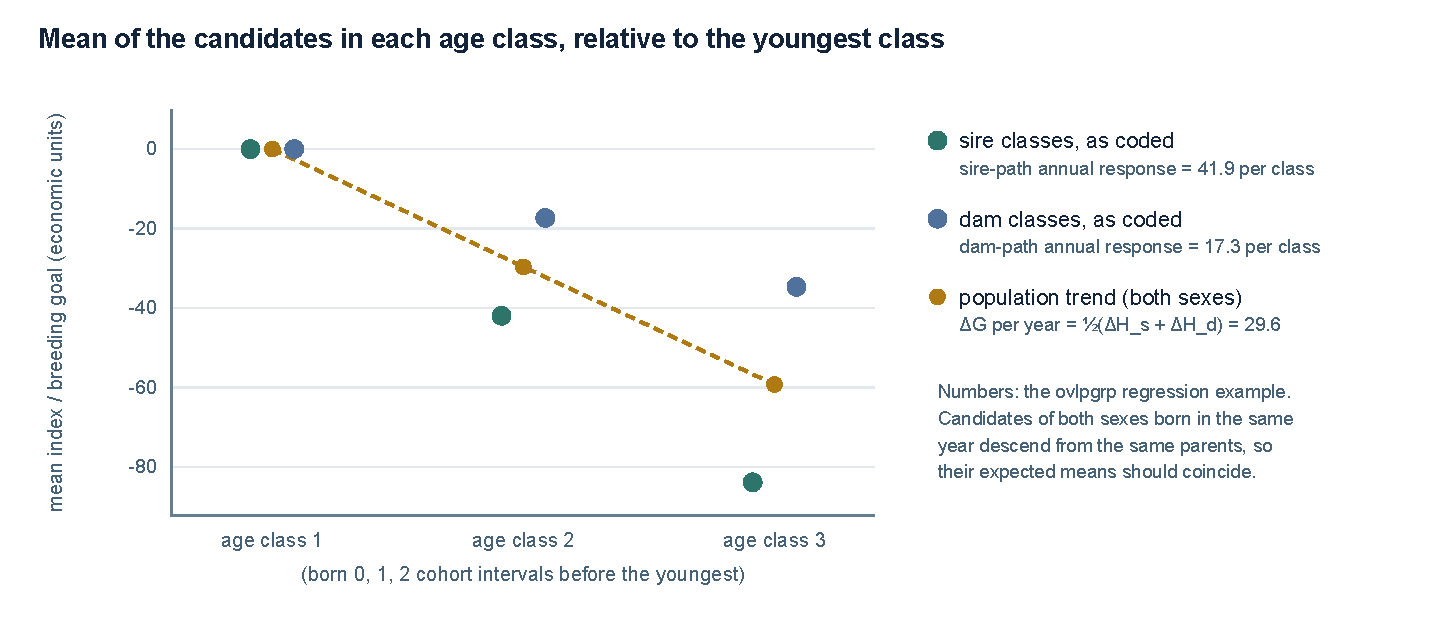
\includegraphics[width=\linewidth]{fig_agelag.pdf}
\caption{Mean of each age class relative to the youngest, as coded (separately per sex) and under the population trend, for the \src{ovlpgrp} example.}\label{fig:agelag}
\end{figure}

We ran both lags through the program (Table~\ref{tab:lag}): (A) the population gain in the threshold search, (B) the population gain per trait in the covariance mixture, and both together.

\begin{table}[ht]
\centering\small
\caption{Effect of using the population gain as the lag. $n$: selected from sire class 1/2 and dam class 1/2. Responses are annual, in economic units.}\label{tab:lag}
\setlength{\tabcolsep}{4pt}
\begin{tabular}{llcccc}\toprule
Example & Lag used & $n$ selected & $L$ & $\Delta G^{\mathrm{year}}$ & $\sigma_H^2$\\\midrule
\src{ovlp2} & as coded & 9.97/0.03/46.20/3.80 & 1.04 & 18.173 & 570.3\\
 & population, both places & 9.90/0.10/48.13/1.87 & 1.02 & 18.235 & 570.8\\
\src{ovlpgrp} & as coded & 10.00/0.00/194.50/5.50 & 1.01 & 29.626 & 512.1\\
 & population, both places & 9.99/0.01/199.75/0.25 & 1.00 & 29.750 & 512.3\\
specified counts & as coded & fixed & 1.32 & 16.662 & 612.3\\
 & population, both places & fixed & 1.32 & 16.558 & 607.9\\\bottomrule
\end{tabular}
\end{table}

The effect is below 1\% here because in these examples almost all parents come from the youngest class. It grows with the number of age classes and with the share of older parents; in specified-count mode, where older classes contribute by design, the effect on the variance is already visible.

\begin{question}{Question 2}
Should the lag between age classes be the population gain $\Delta G^{\mathrm{year}}$ (per trait, $\tfrac12(\Delta A_{s,a}^{\mathrm{year}}+\Delta A_{d,a}^{\mathrm{year}})$) for both sexes, or is there a reason for the per-sex path response?
\end{question}
\begin{recommend}
Use the population gain in both places. We think this follows from the shared birth-cohort mean. We have not changed it, because it is a model choice rather than a programming error.
\end{recommend}

\subsection{Question 3: the former search range and clamp}
Two limits in the original code bounded how intense selection across age classes could be. The Ridders search for $x_g$ in Eq.~\eqref{eq:agecount} was bracketed by $\pm1.5\sqrt{V_{I,g,c}}$ around each class mean, so it could never select fewer than $\bar\Phi(1.5)=6.7\%$ of the youngest class; when more intense selection was needed the root was not bracketed, the search gave up silently, and the selected numbers no longer added up to $M_g$. And the standardised truncation point $(x_g-m_{g,c})/\sqrt{V_{I,g,c}}$ was clamped to $[-3,3]$, so every age class always contributed at least $\bar\Phi(3)=0.135\%$ of its animals. The clamp may have protected the old quadrature for $\bar\Phi$, which broke down beyond about 4 standard deviations (it was off by orders of magnitude beyond 5). The clamp is now removed, the tail uses \src{erfc}, and the search covers $\pm8$ standard deviations.

\begin{table}[ht]
\centering\small
\caption{\src{ovlpgrp} with 1000 young and 500 older sire candidates, as the number of sires varies, before and after removing the clamp (the search range was already widened). These exploratory runs predate correction of a generation-interval error in the modernized fork, so their responses are not an isolated estimate of the clamp's effect. BG: breeding-goal variance; acc.: accuracy of the young-sire index; response: total annual response in the first trait.}\label{tab:clamp}
\begin{tabular}{rcccc}\toprule
& \multicolumn{2}{c}{before} & \multicolumn{2}{c}{after}\\\cmidrule(lr){2-3}\cmidrule(lr){4-5}
Sires & young / old & BG, acc., response & young / old & BG, acc., response\\\midrule
1 & 1.350 / 0.675 & 595.7, 0.746, 5.18 & 1.000 / 0.000 & 510.2, 0.704, 6.98\\
5 & 4.325 / 0.675 & 549.3, 0.725, 5.64 & 5.000 / 0.000 & 511.4, 0.705, 6.25\\
10 & 9.325 / 0.675 & 526.9, 0.713, 5.58 & 10.000 / 0.000 & 512.1, 0.705, 5.91\\
40 & 39.325 / 0.675 & 515.2, 0.707, 5.05 & 39.965 / 0.035 & 514.3, 0.706, 5.13\\
100 & 99.224 / 0.776 & 516.9, 0.708, 4.50 & identical & identical\\\bottomrule
\end{tabular}
\end{table}

In the one-sire row, the former clamp selected 2.025 sires rather than the requested one; the old and new responses therefore do not describe the same selection program. The forced 0.675 older sires also change the covariance mixture. We include this table to show the invalid selected counts and the direction of the numerical effect, not as a clean estimate of the response change from removing the original limits.

\begin{question}{Question 3}
Were the $\pm1.5$ standard-deviation bracket and the $\pm3$ clamp deliberate parts of the model, or numerical safeguards? Does the new behaviour in Table~\ref{tab:clamp} agree with what you would expect?
\end{question}
\begin{recommend}
Keep them removed. They look like safeguards for the old quadrature, and with an exact tail they are no longer needed.
\end{recommend}

\subsection{Question 4: family structure under overlapping generations}
In discrete generations the intensity used for the response is corrected for the correlation between the index values of sibs (the routine \src{rawl3}, after Rawlings \cite{rawlings1976} and Meuwissen \cite{meuwissen1991}). The original SelAction program description also says that intensity is adjusted for each sex-age class under overlapping generations, using Meuwissen's method. In \src{ovlp}, \src{selection\_index} evaluates \src{rawl3} for every active class, but \src{ovlp} then recomputes the responses from the uncorrected $i=\phi(t)/p$, so the correction is discarded. The original source does the same, so this is not a change made in the fork, but it appears to conflict with the program description.

\begin{question}{Question 4}
Was the per-class family-structure correction described in the original program description intended to enter overlapping-generation response? If so, how should it be applied when age classes share a common truncation point?
\end{question}
\begin{recommend}
Retain the current calculation while we establish the intended correction; meanwhile, document the discrepancy with the program description.
\end{recommend}

%======================================================================
\section{Multistage selection}\label{sec:multistage}

\subsection{How the program models multistage selection}
With $m=2$ or 3 stages, each stage has its own index $I_j$, using all information available up to that stage. Candidates must pass every stage; with standardised indices $Z_j$ and correlation matrix $\ma R$, the truncation points satisfy $\Pr(Z_1>t_1)=p_1$, $\Pr(Z_1>t_1,Z_2>t_2)=p_1p_2$, and so on. The mean of the stage indices among the finally selected is the truncated-normal mean of Tallis \cite{tallis1961}:
\begin{equation}\label{eq:tallis}
\E[Z_j\mid\text{all pass}]=\frac{1}{P}\sum_{\ell=1}^m r_{j\ell}\,\phi(t_\ell)\,
\Pr\!\big(Z_k>t_k\ \forall k\ne\ell \,\big|\, Z_\ell=t_\ell\big),
\end{equation}
where $P$ is the overall fraction selected. For three stages the conditional probability in each term is a bivariate normal tail with standardised thresholds $t_{k\mid\ell}=(t_k-r_{\ell k}t_\ell)/\sqrt{1-r_{\ell k}^2}$ and partial correlation
\begin{equation}\label{eq:partial}
r_{jk\mid\ell}=\frac{r_{jk}-r_{j\ell}r_{k\ell}}{\sqrt{(1-r_{j\ell}^2)(1-r_{k\ell}^2)}} .
\end{equation}
The response in each trait is then obtained by regressing the breeding values on the vector of stage indices.

\subsection{Question 5: the stage correlations, $r_{13\mid2}$ and the 0.93 cap}
The program approximates the correlation between stage indices by the ratio of accuracies, caps it at 0.93, and in three-stage selection sets one of the three partial correlations to zero:
\begin{lstlisting}
corrsrih12=srih/srih2          ! r12 = rIH,1 / rIH,2, then capped at 0.93
corrsrih13=srih/srih3          ! r13, capped at 0.93
corrsrih23=srih2/srih3         ! r23, capped at 0.93
dumcorrsrih123=(corrsrih12-corrsrih13*corrsrih23)/((sqrt(1-corrsrih13**2))*(sqrt(1-corrsrih23**2)))
dumcorrsrih132=0.0             ! r13|2
dumcorrsrih231=(corrsrih23-corrsrih12*corrsrih13)/((sqrt(1-corrsrih12**2))*(sqrt(1-corrsrih13**2)))
\end{lstlisting}

\paragraph{The ratio of accuracies is exact here.} If each stage index is the best linear predictor of $H$ from its information $\ve x_j$, and the information is nested ($\ve x_1\subseteq\ve x_2\subseteq\ve x_3$, which the input routine enforces), then $\Cov(\ve x_j,H-I_\ell)=0$ for $j\le\ell$, so $\Cov(I_j,I_\ell)=\Var(I_j)$ and
\[
r_{j\ell}=\frac{\sigma_{I_j}}{\sigma_{I_\ell}}=\frac{r_{IH,j}}{r_{IH,\ell}} .
\]
All stages are evaluated with the same equilibrium covariances, so the condition holds; the printed index variances reproduce all three accuracies against a single $\sigma_H^2$.

\paragraph{So is $r_{13\mid2}=0$.} With the ratio, $r_{12}r_{23}=(\sigma_1/\sigma_2)(\sigma_2/\sigma_3)=r_{13}$, so the numerator of Eq.~\eqref{eq:partial} for $r_{13\mid2}$ is exactly zero: given the stage-2 index, stages 1 and 3 are conditionally independent. Setting it to zero is therefore correct, and presumably why it was done.

\paragraph{The cap breaks this.} If one correlation is capped and the others are not, $r_{12}r_{23}\ne r_{13}$ and the true $r_{13\mid2}$ is no longer zero. The cap binds in both of our multistage regression examples: the uncapped stage correlations were 0.977 (two stages) and 0.971, 0.870, 0.896 (three stages). With $r_{12}$ capped at 0.93 the partial correlation should be 0.224, not 0. We compared the program as coded with (A) $r_{13\mid2}$ computed from Eq.~\eqref{eq:partial} and with an exact model in which thresholds are solved exactly and nothing is capped.

\begin{table}[ht]
\centering\small
\caption{Three-stage selection: total sire response after stage 3 (economic units) for variants of the \src{test3s} example. Errors are relative to the exact model.}\label{tab:stage3}
\begin{tabular}{lccccc}\toprule
Sire fractions per stage & as coded & (A) & no cap & error as coded & error with (A)\\\midrule
0.5 / 0.2 / 0.1 (\src{test3s}) & 18.112 & 18.112 & 18.112 & $-0.00\%$ & $+0.00\%$\\
0.1 / 0.5 / 0.2 & 17.778 & 18.046 & 18.041 & $-1.45\%$ & $+0.03\%$\\
0.02 / 0.5 / 0.5 & 17.849 & 18.873 & 18.843 & $-5.30\%$ & $+0.13\%$\\
0.05 / 0.2 / 0.5 & 18.553 & 18.879 & 18.867 & $-1.68\%$ & $+0.05\%$\\\bottomrule
\end{tabular}
\end{table}

For one case we also checked Eq.~\eqref{eq:tallis} itself against direct numerical integration of the conditional normal: with the computed $r_{13\mid2}$ the means agree to $4\times10^{-9}$, with $r_{13\mid2}=0$ they are off by $4\times10^{-5}$.

\paragraph{Why not remove the cap?} The cap appears to protect the numerical integration. The bivariate and trivariate normal probabilities are computed with Dutt's integral representation \cite{dutt1973} and Gauss--Hermite quadrature, whose accuracy deteriorates as the correlation approaches 1: in the cases tested, we measured a maximum relative error of $2.5\times10^{-5}$ up to $r=0.93$, $5\times10^{-4}$ at 0.97, and complete failure at 0.99. In a two-stage example with an uncapped correlation of 0.9998, raising the cap to 0.99 gave 2.5 times, and removing it 7.6 times, the reference response. Where the integration worked in our examples, the cap changed response by up to about 1.7\%.

\begin{question}{Question 5}
Was the 0.93 cap introduced for the numerical integration, as it appears? Do you agree that with nested best-linear-predictor indices the ratio of accuracies is the intended correlation, and that $r_{13\mid2}$ should then be computed from Eq.~\eqref{eq:partial} rather than set to zero?
\end{question}
\begin{recommend}
Compute $r_{13\mid2}$ from Eq.~\eqref{eq:partial}: it gives the same result whenever the cap does not bind, and removed a response difference of up to 5.3\% in the cases tested when it did. Keep the 0.93 cap until the bivariate and trivariate normal integrals are replaced by a method accurate for correlations near 1, such as Genz's \cite{genz2004}; then reassess the cap.
\end{recommend}

\subsection{Question 6: half-sib information when each sire has one dam}
Under SelAction's balanced, nested mating assumption, $M_s=M_d$ means one dam per sire, so there are no paternal half sibs from other dams in that mating cohort. The program says so (``half-sib information is thus not possible, and will be removed'') and removes half-sib sources, but only from the final-stage index. A half-sib group given as an earlier-stage source stays in that stage's index and receives large weights. In a two-stage example with 50 sires and 50 dams and a half-sib group at stage 1, the half-sib group got index weights of 1.08 and $-5.45$ on two traits, raising stage-1 accuracy from 0.508 to 0.537 and stage-1 response by 5.6\%. The final-stage response was unaffected in this example.

A related point: the program never checks the number of dams in a half-sib group against the mating ratio. If that group is restricted to offspring of the candidate's sire from the same mating cohort, $m_H\le d-1$ would follow. Our own three-stage regression example uses half-sib groups of 200 dams with 20 dams per sire, and the program accepts it. This inequality depends on the intended group definition.

\begin{question}{Question 6}
Should half-sib sources be removed from every stage when $M_s=M_d$? And what is the intended meaning of the number of dams in a half-sib group: should it be limited to $d-1$, or can a half-sib group be defined more widely?
\end{question}
\begin{recommend}
Apply the program's mating-ratio-one rule to every stage. Clarify whether half-sib group dams must come from the current sire's $d$ matings before adding a group-size warning.
\end{recommend}

%======================================================================
\section{Rate of inbreeding}\label{sec:inbreeding}

\subsection{How the program predicts the rate of inbreeding}
The rate of inbreeding in one-stage discrete selection follows Bijma and Woolliams \cite{bijmawoolliams2000}: expected long-term contributions are obtained from the selective advantage of the parents, and a correction for finite family sizes is added. The correction (routines \src{Poissoncorr} and \src{hyper\_correct}) uses co-selection probabilities of sibs in the manner of Burrows, as reappraised by Wray, Woolliams and Thompson \cite{wray1990}. For a pair of sibs of sexes $u$ and $v$ with intra-class correlation $\rho_{uv}$ of their index values, the program approximates the ratio of the probability that a sib is selected given that the other one is, to the unconditional probability, as
\begin{equation}\label{eq:kappa}
\kappa_{uv}=\frac{1}{p_v}\,\Phi\!\left(\frac{i_u\rho_{uv}-t_v}{\sqrt{1-k_u\rho_{uv}^2}}\right),
\end{equation}
and six such ratios (full and half sibs; male--male, male--female, female--female) give the variances of family sizes. Before this, each sample correlation is adjusted for finite population size,
\[
\rho \leftarrow \rho-\rho(1-\rho^2)\left(\frac{a}{M_s}+\frac{b}{M_d}\right),\qquad
(a,b)=\begin{cases}(0.8634,\,0.954)&\text{full sibs},\\(1.4075,\,1.4581)&\text{half sibs}.\end{cases}
\]

\subsection{Question 7: the hard switch in the inbreeding correction at 20 sires}
With fewer than 20 sires the selected fractions used in Eq.~\eqref{eq:kappa} are first adjusted. The code says this follows Wray et al.\ (1990) as used in Bijma and Woolliams (2000):
\begin{lstlisting}
!correction of the selected proportion according to Wray et al., 1990
 IF(m<20) THEN
      pmfs=(1.0-rhofsmm)*pm + rhofsmm*MAX(pm,1.0/REAL(m))
      pffs=(1.0-rhofsff)*pf + rhofsff*MAX(pf,1.0/REAL(m))
      pmhs=(1.0-rhohsmm)*pm + rhohsmm*MAX(pm,1.0/REAL(m))
      pfhs=(1.0-rhohsff)*pf + rhohsff*MAX(pf,1.0/REAL(m))
\end{lstlisting}
(\src{m} is $M_s$, \src{f} is $M_d$.) That is, for a sib pair of sex $g$,
\[
p_g^{*}=(1-\rho_{gg})\,p_g+\rho_{gg}\max\!\left(p_g,\frac{1}{M_s}\right),
\]
for males \emph{and} females. This is Eq.~13 of Bijma and Woolliams \cite{bijmawoolliams2000}, $p_{x,\mathrm{adj}}=(1-\rho_{\mathrm{fam}})p_x+\rho_{\mathrm{fam}}\max(p_x,1/N_m)$, written for either sex $x$ with $N_m$ the number of sires. The paper describes it as a weighted sum of the original selected proportion and the selected proportion when selecting between families, since with large $\rho_{\mathrm{fam}}$ selection moves towards between-family selection. So $1/M_s$ for females is the published form, not a slip.

The mixed (male--female) pairs take $i,k$ from the adjusted male fraction and $t,p$ from the adjusted female fraction, so the adjustment affects them too.

The remaining question is the hard switch. At 20 sires two things change at once: the adjustment above is turned off, and \src{hyper\_correct} adds the $\beta$ terms of the long-term contributions. In a one-stage variant of \src{test1} with 50 dams, 5 male and 20 female candidates per dam ($p_f=0.05$, $p_s=M_s/250$), predicted $\Delta F$ rises from 4.590\% at 19 sires to 4.682\% at 20 (Figure~\ref{fig:deltaf}). The header of \src{dFmtblup} notes that a discontinuity may occur. Bijma and Woolliams applied the selected-fraction adjustment for schemes with 5 or 10 sires, and in one extreme 20-sire scheme ($d=10$, $n_o=16$, $h^2=0.1$) showed that it reduced a 37\% overprediction to $-13$\%. The paper does not state a cutoff at 20 sires. The same code is in the original source.

\begin{figure}[ht]
\centering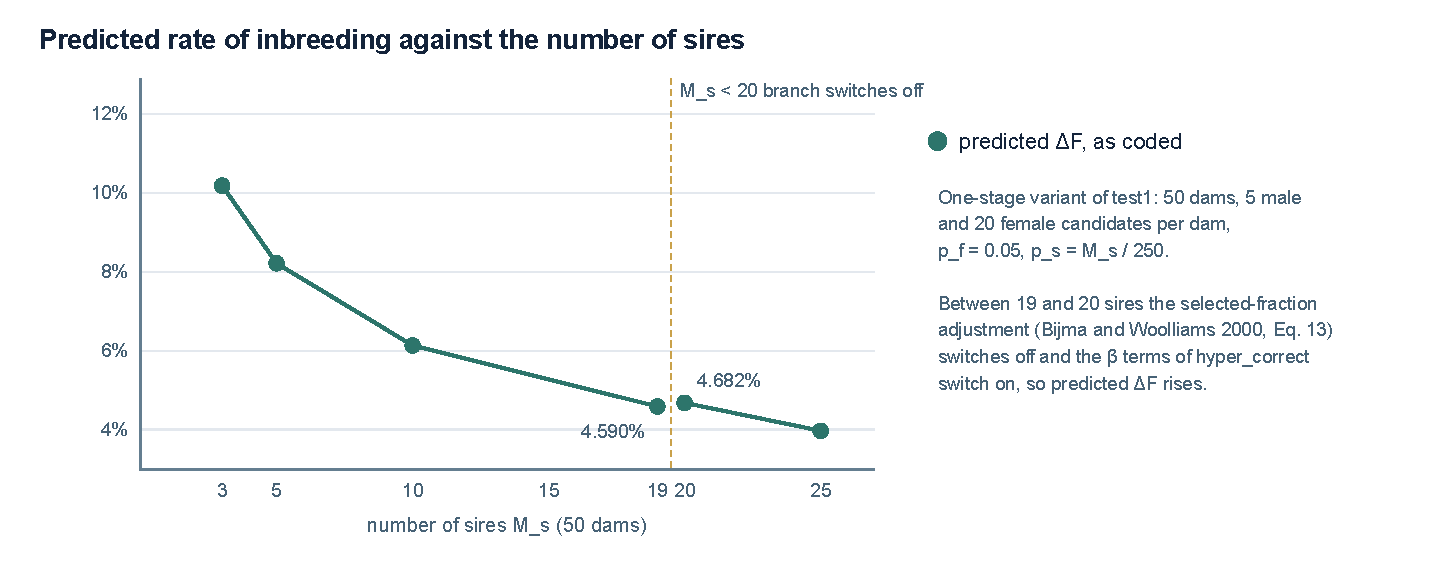
\includegraphics[width=\linewidth]{fig_deltaf.pdf}
\caption{Predicted rate of inbreeding against the number of sires, as coded, showing the rise between 19 and 20 sires.}\label{fig:deltaf}
\end{figure}


\begin{question}{Question 7}
What motivated the cutoff at $M_s<20$ and the simultaneous addition of the $\beta$ terms at $M_s=20$? Is the resulting rise in $\Delta F$ acceptable for users comparing breeding schemes near that boundary?
\end{question}
\begin{recommend}
Keep the published $1/M_s$ adjustment. Document the discontinuity and investigate the two switches separately before changing either threshold.
\end{recommend}

%======================================================================
\section{Numerical points, for information}\label{sec:numerics}
These need no decision.
\begin{itemize}
\item \textbf{Unreproduced BLUP/group response report.} An earlier project note reported zero response when BLUP was combined with groups under overlapping generations, but the triggering input was not saved and a 72-input sweep did not reproduce it. No model question is raised on this basis.
\item \textbf{Asymmetry of the EBV covariance matrices.} The starting values of the sire and dam EBV covariance matrices $\ma S,\ma D$ use $h_q^2\Cov(A_p,A_q)$, which is not symmetric when heritabilities differ, and the update carries the asymmetry forward. It decays by about a factor of three per round and is at rounding level by round 13 of 25, so it does not affect the reported results; making the matrices symmetric changes no output. We may symmetrise them anyway for clarity.
\item \textbf{Tolerance of the multistage threshold search.} The Newton search stops when the selected fraction is within $10^{-5}$ in absolute terms, which is coarse for small fractions (0.2\% relative at $p=0.005$, worth about 0.1\% of response). It now prints a warning when it does not converge within its 20 steps; before, non-convergence was silent.
\item \textbf{One-round lag under overlapping generations.} Each class's phenotypic covariance matrix is rebuilt from the additive matrix of the previous round. This has no effect at convergence.
\end{itemize}

%======================================================================
\section{What we would do next}
Depending on your answers: compute $r_{13\mid2}$ (Question~5); apply the mating-ratio-one half-sib rule at all stages (Question~6); and assess the age-class lag (Question~2), family-structure correction (Question~4), and 20-sire switch (Question~7). We would first establish the intended group definition before adding a group-size warning. Each change would be documented with before-and-after results on the regression examples. Replacing the bivariate and trivariate normal integration would follow, after which the 0.93 cap could be reassessed.

We would be grateful for any answers, partial or not, and for pointers to derivations or notes from the original development, in particular for the inbreeding correction.

%======================================================================
\begin{thebibliography}{99}
\bibitem{bijmawoolliams2000} Bijma, P. and J.A. Woolliams. 2000. Prediction of rates of inbreeding in populations selected on best linear unbiased prediction of breeding value. \emph{Genetics} 156:361--373. \href{https://doi.org/10.1093/genetics/156.1.361}{doi:10.1093/genetics/156.1.361}
\bibitem{dutt1973} Dutt, J.E. 1973. A representation of multivariate normal probability integrals by integral transforms. \emph{Biometrika} 60:637--645. \href{https://doi.org/10.1093/biomet/60.3.637}{doi:10.1093/biomet/60.3.637}
\bibitem{genz2004} Genz, A. 2004. Numerical computation of rectangular bivariate and trivariate normal and $t$ probabilities. \emph{Statistics and Computing} 14:251--260. \href{https://doi.org/10.1023/B:STCO.0000035304.20635.31}{doi:10.1023/B:STCO.0000035304.20635.31}
\bibitem{hill1974} Hill, W.G. 1974. Prediction and evaluation of response to selection with overlapping generations. \emph{Animal Production} 18:117--139. \href{https://doi.org/10.1017/S0003356100017372}{doi:10.1017/S0003356100017372}
\bibitem{meuwissen1991} Meuwissen, T.H.E. 1991. Reduction of selection differentials in finite populations with a nested full--half sib family structure. \emph{Biometrics} 47:195. \href{https://doi.org/10.2307/2532506}{doi:10.2307/2532506}
\bibitem{rawlings1976} Rawlings, J.O. 1976. Order statistics for a special class of unequally correlated multinormal variates. \emph{Biometrics} 32:875. \href{https://doi.org/10.2307/2529271}{doi:10.2307/2529271}
\bibitem{rendel1950} Rendel, J.M. and A. Robertson. 1950. Estimation of genetic gain in milk yield by selection in a closed herd of dairy cattle. \emph{Journal of Genetics} 50:1--8. \href{https://doi.org/10.1007/BF02986789}{doi:10.1007/BF02986789}
\bibitem{tallis1961} Tallis, G.M. 1961. The moment generating function of the truncated multi-normal distribution. \emph{Journal of the Royal Statistical Society B} 23:223--229. \href{https://doi.org/10.1111/j.2517-6161.1961.tb00408.x}{doi:10.1111/j.2517-6161.1961.tb00408.x}
\bibitem{wray1990} Wray, N.R., J.A. Woolliams and R. Thompson. 1990. Methods for predicting rates of inbreeding in selected populations. \emph{Theoretical and Applied Genetics} 80:503--512. \href{https://doi.org/10.1007/BF00226752}{doi:10.1007/BF00226752}
\end{thebibliography}

%======================================================================
\appendix
\section{Programming errors already fixed}\label{app:fixed}
For completeness, the other corrections made since the original code, none of which raises a modelling question. Unless stated, they do not change any result on the regression examples.
\begin{itemize}
\item Overlapping generations crashed: two arrays were used before being allocated.
\item Uninitialised values: the progeny-test common-environment fraction (read only when both progeny groups and common environment are requested, but always used; this one did change index weights when memory held other values), a BLUP flag in the four information-source routines, the group-size arrays, and a starting index variance.
\item Divisions by zero for group types that are not configured, a square root of a transiently negative index variance, and a division by zero in \src{rawl3} at a correlation of exactly 1.
\item Two-stage selection with $M_s=M_d$ left the mean dam-EBV sources of half-sib groups in the final index (with zero weight).
\item Warnings added: when the requested number of parents cannot be selected under overlapping generations; when the multistage threshold search does not converge; and when an overlapping-generation index has a trait without phenotypic information and without genetic correlation to one that has.
\item ``\% of total response'' prints \texttt{n/a} instead of dividing by a near-zero total.
\end{itemize}

\section{Reproducing the numbers}
The current ``as coded'' results use \src{fortran\_mac/} at commit \src{dbdd69f} with GNU Fortran 14.2.0. The exploratory clamp comparison in Table~\ref{tab:clamp} predates the fork's generation-interval correction, as noted in its caption. Alternatives were run in scratch copies; the uncapped multistage reference also changed the threshold and probability calculations as described in Question~5. The seven regression inputs are in \src{tests/fixtures/}. Other runs varied parent counts, selected fractions, or information sources as stated in the tables; those scratch inputs and modified sources are not part of the repository.
\end{document}
